\section{Results}

\medskip
\noindent\textit{Part 1: Does the separation happen, and what creates it?}

\subsection{What creates the separation}

We decompose the contribution of the two devices we add --- the horizon gate and the cross-covariance penalty --- by switching each on and off. The mechanism-free cell (Section~\ref{sec:xcov}) is also the baseline in which only the coordinate split remains.

\begin{table}[!tbp]
\caption{Separation index by mechanism. Cells are SEP (higher is better), $n=5$ seeds, $\lambda=4$. Bold marks the best cell in each row. The gate and the penalty are complementary: neither alone reaches what the two reach together.}
\label{tab:ablation}
\centering
\small
\begin{tabular}{llcccc}
\hline
Dataset & Stem & Neither & Gate only & xcov only & \textbf{Gate + xcov} \\
\hline
Synthetic & Reg & 0.135 & 0.342 & 0.279 & \textbf{0.408} \\
Synthetic & NCE & 0.121 & 0.124 & 0.488 & \textbf{0.749} \\
PTB-XL & Reg & 0.375 & 0.404 & 0.312 & \textbf{0.495} \\
PTB-XL & NCE & 0.392 & 0.503 & 0.283 & \textbf{0.567} \\
HAPT & Reg & 0.521 & 0.537 & 0.236 & \textbf{0.632} \\
HAPT & NCE & 0.297 & 0.366 & 0.162 & \textbf{0.515} \\
\hline
\end{tabular}
\end{table}

In Table~\ref{tab:ablation} the model with both devices ranks first in all six settings, and neither device alone reaches that value. On the contrastive stem of the synthetic data the gate alone is indistinguishable from the mechanism-free case (0.124 against 0.121), yet adding that same gate to the penalty raises SEP from 0.488 to 0.749: the two devices need each other. The penalty alone is actively harmful on the real data, breaking down the inclusion term and falling below even the mechanism-free case.

The ``Neither'' cells take the first 16 of the 64 dimensions, and their SEP agrees in all six settings to within 0.015 with the SEP of 16 dimensions drawn at random from the same embedding. Without our devices, any part of the embedding holds the two factors to a similar degree, so coordinate position carries no meaning by itself; our contribution is to give those coordinates structure.

\subsection{Separation requires a latent target}

This section ablates a third design axis, the \emph{target space}, testing the premise of the latent-prediction family: that prediction should be made in a latent space rather than on the raw signal. We hold the gate, the anchor, the horizon and the loss form fixed and change only what is predicted. The latent target is the 64-dimensional output the target encoder reads from the future interval; the raw target is the patch itself at that time (with one extra linear head). Both models carry the cross-covariance penalty, so $\lambda$ has the same meaning for each, and we compare each at its own best value over the swept curve.

\begin{table}[!tbp]
\caption{Latent target against raw target. Cells are SEP on synthetic, $n=5$ seeds, each stem at its own best $\lambda$. Bold marks the latent target. Everything but the prediction target is held fixed.}
\label{tab:latentraw}
\centering
\small
\begin{tabular}{lccc}
\hline
Stem & Latent (best) & Raw (best) & Difference \\
\hline
HGLP-Reg & \textbf{0.809} ($\lambda=1$) & 0.415 ($\lambda=4$) & $+0.394$ ($1.95\times$) \\
HGLP-NCE & \textbf{0.844} ($\lambda=16$) & 0.432 ($\lambda=16$) & $+0.411$ ($1.95\times$) \\
\hline
\end{tabular}
\end{table}



Replacing the latent target with raw patches halves SEP on both stems (Table~\ref{tab:latentraw}); since both carry the same penalty and are compared at their own optimal $\lambda$, neither side gains from the knob. The allocation term is the same for the two targets, at 0.86 to 0.89, and the gap opens in the inclusion term: the raw target loses the persistent factor as the penalty grows, falling from 0.807 to 0.401, whereas the latent target stays above 0.97 throughout. The raw signal still contains the transient component, and the pressure to predict it too pushes out the persistent factor. The gate and the penalty of Section~IV-A are thus not enough on their own; the latent target has to be present as well.

\subsection{Can post-hoc processing take its place?}

If an embedding trained without the gate is rotated post-hoc without labels --- by principal component analysis, by slowness-ordered independent component analysis, or by slow feature analysis (SFA) --- does it reach the same separation? These methods need no horizon gate at all, so they are the sharpest objection to our method.

\begin{table}[!tbp]
\caption{Our method against label-free post-hoc unmixings. Cells are SEP, $n=5$ seeds. Our method has one knob, so we report its best point on the swept $\lambda$ curve; each unmixing is a single fixed value. Bold marks the winner of each row. The verdict is three to three overall: two of two on synthetic, one of four on real data.}
\label{tab:rotation}
\centering
\small
\begin{tabular}{llccc}
\hline
Dataset & Stem & Ours (best $\lambda$) & SFA & Verdict \\
\hline
Synthetic & Reg & \textbf{0.814} ($\lambda=1$) & 0.446 & win \\
Synthetic & NCE & \textbf{0.849} ($\lambda=16$) & 0.388 & win \\
PTB-XL & Reg & 0.495 & \textbf{0.567} & loss \\
PTB-XL & NCE & 0.567 & \textbf{0.599} & loss \\
HAPT & Reg & 0.677 & \textbf{0.717} & loss \\
HAPT & NCE & \textbf{0.626} ($\lambda=64$) & 0.527 & win \\
\hline
\end{tabular}
\end{table}

\begin{figure}[!tbp]
\centering
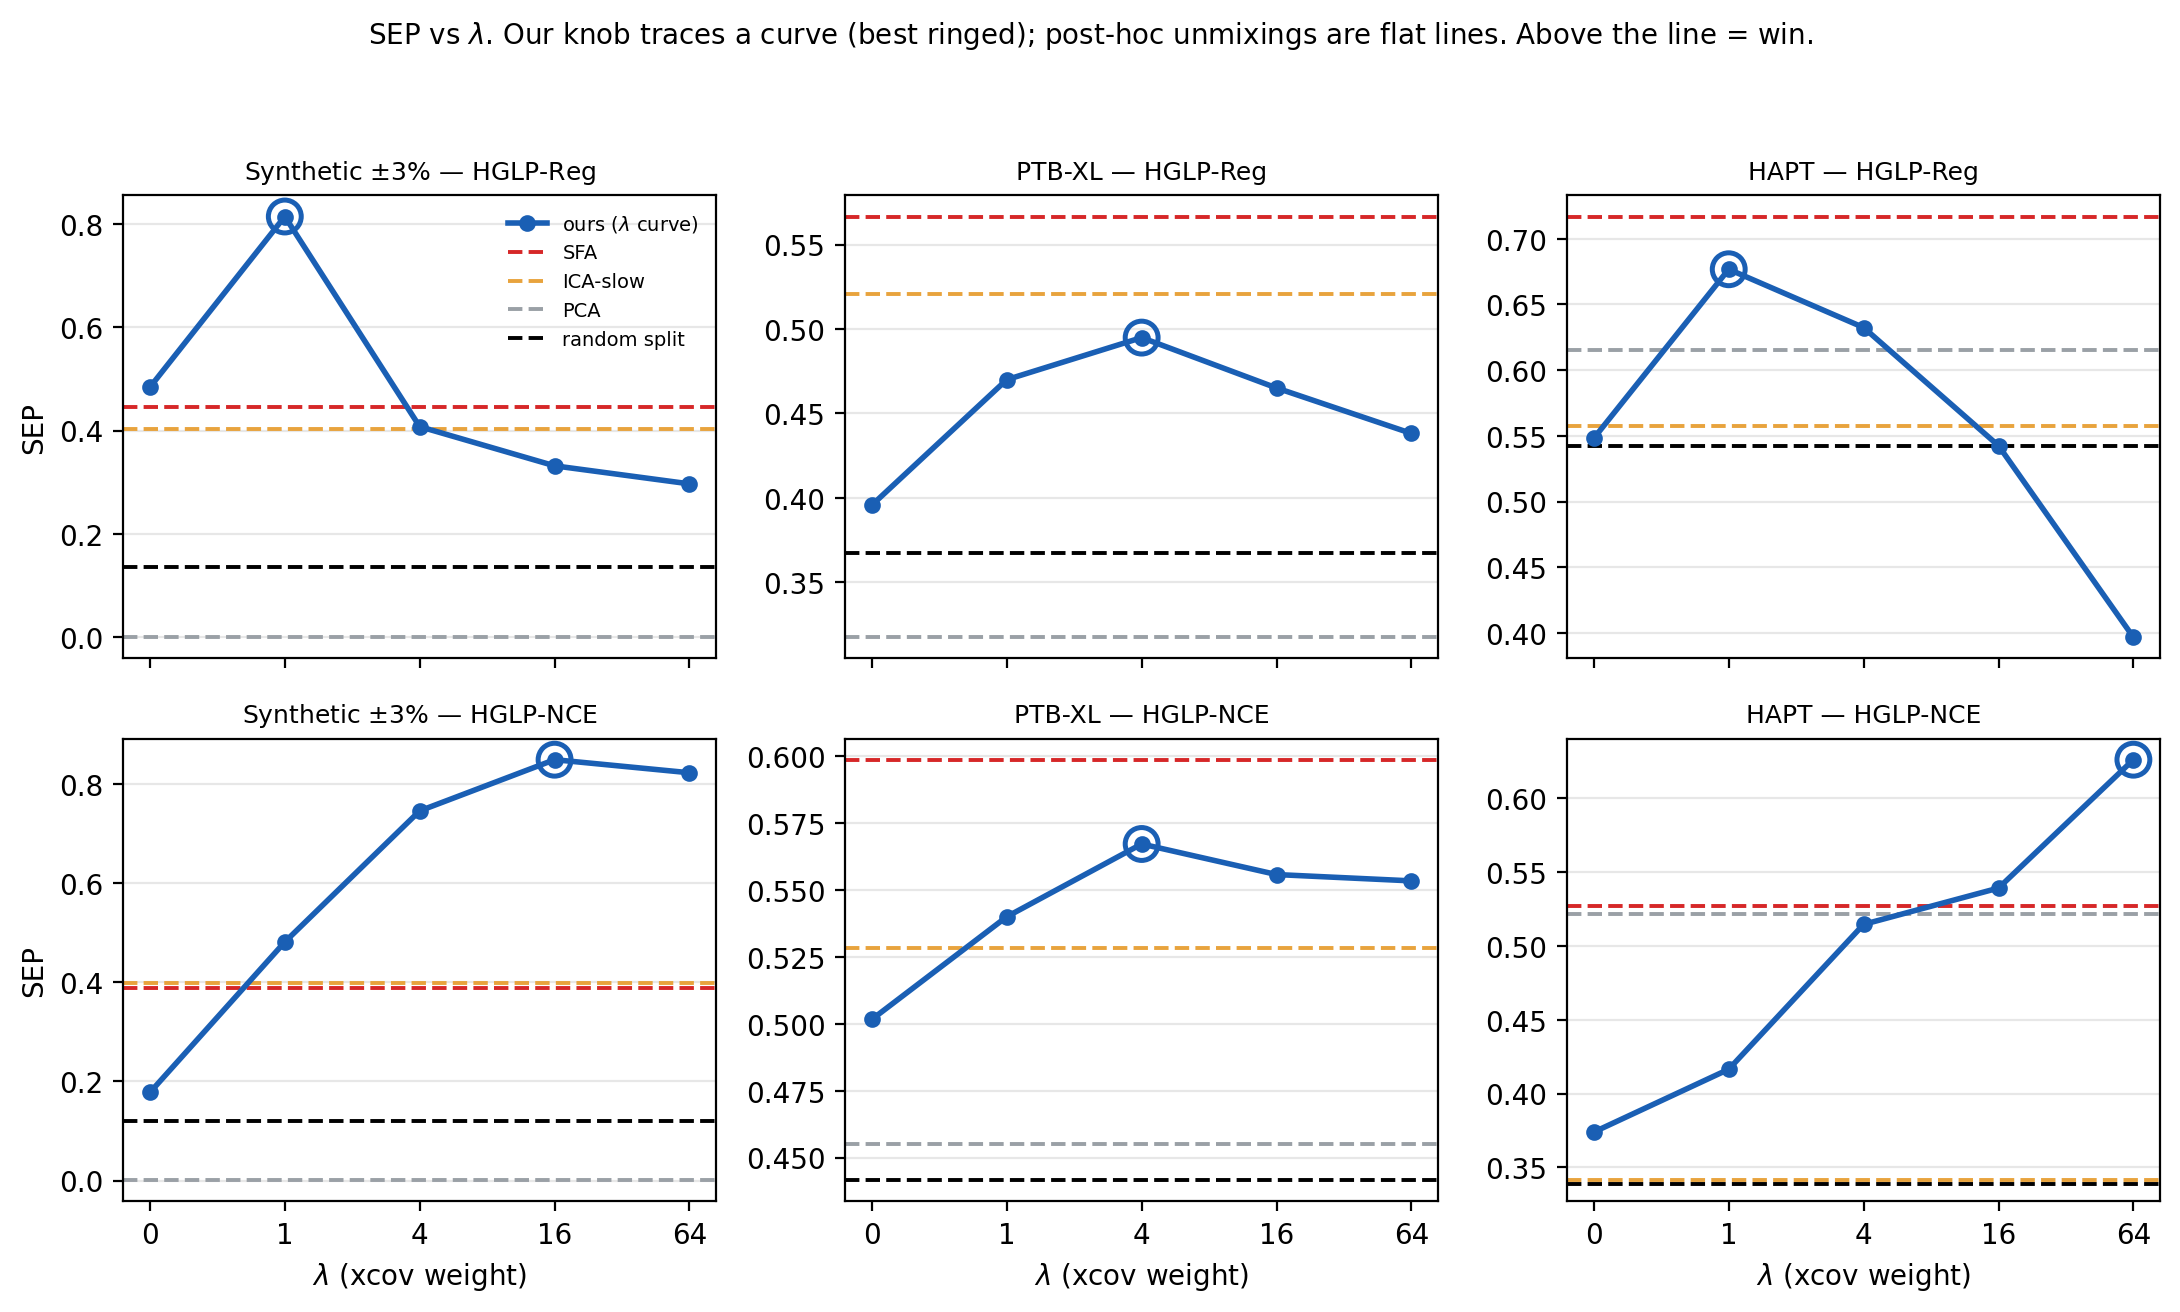
\includegraphics[width=\textwidth]{figs/fig_rotation_sep.png}
\caption{SEP against the penalty weight $\lambda$. $n=5$ seeds. Our method traces a curve over $\lambda\in\{0,1,4,16,64\}$ with its best point ringed; each post-hoc unmixing has no knob and is a horizontal line. A win is our curve rising above the SFA line. Unlike an inclusion--exclusion plane, this view combines all three SEP terms, so it also shows the one real-data win, which the inclusion--exclusion plane cannot display.}
\label{fig:rotation}
\end{figure}

We have one knob and the post-hoc rotations have none, so we report the whole curve rather than a single point (Table~\ref{tab:rotation}, Fig.~\ref{fig:rotation}); only our method has a knob that can be swept, and hiding that asymmetry would not make the comparison fair. On the synthetic data the curve passes above every post-hoc rotation point, and principal component analysis fails completely (SEP 0.000) --- direct evidence that a ranking by variance is not a ranking by persistence, since the transient factor crowds into the leading components and nothing is left in the complement. On the real data we do not lead: SFA reaches the same inclusion at a higher exclusion. The verdict over all six settings is three wins to three losses, but split apart it is two of two on synthetic and three losses of four on real data, with losing margins of 0.032 to 0.072 against a winning margin of 0.099.

This shortfall is expected. Persistence and spectral slowness coincide only under particular assumptions, and our synthetic data deliberately breaks that coincidence: the persistent factor hides inside the oscillation frequency and cannot be reached by low-pass filtering. On PTB-XL and HAPT the persistent factor largely coincides with the slow component, so SFA, which optimizes slowness directly, does the same job by a more direct route --- Section~\ref{sec:coincidence} measures in what sense that coincidence holds, and finds it is not the same sense on the two datasets. Our advantage appears where the two axes come apart; where they coincide, post-hoc rotation already suffices. What remains ours is that the coordinates are fixed during training, so no second fitting stage is needed at deployment --- an operational difference, not a difference in the quality of the separation.

\subsection{Where does that coincidence actually hold?}
\label{sec:coincidence}

The paragraph above is an explanation, and until now it was an unmeasured one. Turning it into a measurement first requires separating two things the word ``slow'' was carrying at once: \textbf{(a)} the factor is legible in the low-frequency \emph{band of the signal}, and \textbf{(b)} some direction of the \emph{representation} changes little over time. SFA optimizes (b) --- under a unit-variance constraint it minimizes the time derivative of its output, which says nothing about where in the spectrum the factor lives. We therefore measure the two separately.

For (a) we filter the raw signal to one band at a time and fit the same linear probe on that band alone (Table~\ref{tab:bandaccess}). Only HAPT clears chance by a real margin, at $\numHaptBandRatio\times$; posture is the DC distribution of gravity across three accelerometer axes, so this is expected. On PTB-XL the low band is \emph{at} chance (\numPtbLowBand{} against \numPtbChance) and the diagnosis lives instead in the 2--5\,Hz QRS morphology. Yet SFA wins on PTB-XL. Sense (a) is therefore not what is happening there, and the single-sentence explanation was incomplete.

\begin{table}[!tbp]
\caption{Is the persistent factor readable from the \emph{slow band of the signal}?
Each row filters the raw signal to one band at a time and fits the same linear probe on
that band alone. Cells are the score named in the second column; ``low band'' is
$0$--$0.5$\,Hz for HAPT (a true low-pass, keeping DC), $0.05$--$0.5$\,Hz for PTB-XL
(band-pass: the ECG baseline is arbitrary), $f<0.02$ for the synthetic carrier. The
ratio column is low band over chance. Only HAPT clears chance by a real margin.}
\label{tab:bandaccess}
\centering
\small
\begin{tabular}{llcccc}
\hline
Dataset & Score & Low band & Chance & Low/chance & Best band (score) \\
\hline
Synthetic & $R^2$ & $8.2\times 10^{-6}$ & 0 & --- & carrier freq.\ (0.279) \\
PTB-XL & macro-F1 & 0.498 & 0.500 & 1.00 & 2.0-5.0\,Hz (0.761) \\
HAPT & macro-F1 & \textbf{0.570} & 0.167 & \textbf{3.42} & 0.0-0.5\,Hz (0.570) \\
\hline
\end{tabular}
\end{table}


For (b) we ask whether ordering the directions of an ungated embedding by slowness \emph{finds} the persistent factor, and by how much:
\begin{equation}
C=\frac{s_{\text{per}}(\text{SFA's slow half}) - s_{\text{per}}(\text{random 16})}
       {s_{\text{per}}(\text{full 64}) - s_{\text{per}}(\text{random 16})}.
\label{eq:metricC}
\end{equation}
All three terms are read off one mechanism-free embedding --- gate, penalty and per-block LayerNorm all absent --- re-based three ways, so they are already stored in the runs of Table~\ref{tab:rotation} and need no retraining. The full 64 dimensions are a genuine ceiling: fitting a probe inside a 16-dimensional subspace is the same optimization restricted to that subspace, and a restricted optimum cannot beat an unrestricted one. A random 16 is \emph{not} a floor; it is the null reference for ``no ordering at all,'' and subspaces below it certainly exist --- producing one is the point of our method.

\begin{table}[!tbp]
\caption{Does ordering by slowness \emph{find} the persistent factor? All four score
columns are the persistent factor read by a linear probe from a 16-dimensional subspace
of the \emph{same mechanism-free} embedding (macro-F1 on real data, accuracy on
synthetic); only the choice of subspace differs. $C$ is the fraction of the reachable
range $(\text{full}-\text{random})$ that the slowness ordering recovers; $n=5$ seeds,
$\pm$ is the seed standard deviation. \textbf{Read the sign, not the size}: the
denominator is small, so the ratio is noisy, but real data and synthetic data do not
overlap.}
\label{tab:metricC}
\centering
\small
\begin{tabular}{llcccc}
\hline
Dataset & Stem & SFA slow half & Random 16 & Full 64 & $C$ \\
\hline
Synthetic & HGLP-Reg & 0.862 & 0.856 & 0.886 & $\mathbf{-0.22} \pm 0.72$ \\
Synthetic & HGLP-NCE & 0.986 & 0.986 & 0.985 & $\mathbf{-1.49} \pm 1.24$ \\
PTB-XL & HGLP-Reg & 0.770 & 0.750 & 0.778 & $\mathbf{+0.42} \pm 0.73$ \\
PTB-XL & HGLP-NCE & 0.791 & 0.776 & 0.793 & $\mathbf{+0.78} \pm 0.61$ \\
HAPT & HGLP-Reg & 0.898 & 0.881 & 0.920 & $\mathbf{+0.35} \pm 0.59$ \\
HAPT & HGLP-NCE & 0.909 & 0.876 & 0.929 & $\mathbf{+0.56} \pm 0.31$ \\
\hline
\end{tabular}
\end{table}


$C$ is positive in all four real settings and negative in both synthetic ones, with no overlap (Table~\ref{tab:metricC}). The negative sign is the stronger statement: on synthetic data, ordering by slowness is \emph{worse than picking at random}, so slowness does not merely fail to find the persistent factor, it points away from it --- exactly what designing the factor to hide inside the oscillation frequency was meant to produce. Two caveats. The denominator is small, because inclusion is high everywhere, so the ratio is unstable; $C$ should be read as a signed indicator and not as a continuous degree of alignment. And $C$ shares machinery with SFA, since slowness ordering is what SFA does --- it isolates the mechanism by which SFA succeeds rather than testing SFA from outside. It is still not circular: our method appears nowhere in Eq.~\ref{eq:metricC}, and defining alignment as SFA's own SEP would have made the claim ``SFA wins because SFA wins.''

Putting the two metrics together, the one sentence covered two different routes. On HAPT the factor genuinely sits in the slow band. On PTB-XL it does not, but the diagnosis is constant over an entire record, so its time derivative is zero --- the limiting solution of exactly what SFA maximizes. HAPT wins by route (a) and PTB-XL by route (b), and only the synthetic data, where the persistent factor is neither band-slow nor window-constant, is closed to both.

\subsection{Following the exclusion clause through}
\label{sec:exclusion}

Section~\ref{sec:handpicked} states that our objective enforces availability but not exclusion. This section asks what that admission costs in practice, in four steps: where the shortfall against SFA actually sits, whether a structural change removes it, whether it survives a stronger probe, and whether the knob that governs it can be set without labels.

\textbf{The shortfall is entirely on the exclusion term.} SEP is a product of three factors, so a single number cannot say which one is losing. Splitting it and pairing by seed (Table~\ref{tab:terms}) gives an unusually clean answer: inclusion is a draw in all six settings ($\numInclDiffLo$ to $\numInclDiffHi$), every real-data loss is a loss on exclusion alone, and every win is a win on allocation. The method does not degrade diffusely; it degrades on the one term the objective was never able to enforce.

\begin{table}[H]
\caption{Where the shortfall against SFA sits. Cells are \emph{ours minus SFA} on one
term of SEP, paired by seed then averaged, $n=5$; positive means we lead, and our column is
taken at the listed $\lambda$.}
\label{tab:terms}
\centering
\small
\begin{tabular}{lllcccc}
\hline
Dataset & Stem & $\lambda$ & Inclusion & Allocation & Exclusion & SEP \\
\hline
Synthetic & HGLP-Reg & 1 & $+0.102$ & $+0.236$ & $+0.156$ & $+0.395$ \\
Synthetic & HGLP-NCE & 16 & $-0.006$ & $+0.327$ & $+0.266$ & $+0.451$ \\
PTB-XL & HGLP-Reg & 4 & $-0.007$ & $+0.048$ & $\mathbf{-0.136}$ & $-0.073$ \\
PTB-XL & HGLP-NCE & 4 & $-0.000$ & $+0.007$ & $\mathbf{-0.051}$ & $-0.031$ \\
HAPT & HGLP-Reg & 1 & $-0.033$ & $-0.011$ & $-0.007$ & $-0.039$ \\
HAPT & HGLP-NCE & 64 & $-0.041$ & $+0.155$ & $-0.016$ & $+0.100$ \\
\hline
\end{tabular}
\end{table}


\textbf{The asymmetry of the gate is a design choice, not an oversight.} If exclusion is the weak term, the obvious repair is structural: also switch $\zslow$ \emph{off} below $\tau$, by multiplying it by $1-g(\Delta)$, so that no horizon is ever in a position to push transient information into it. We retrained all six settings that way, five values of $\lambda$ and five seeds each. The symmetric variant is better in \numSymBetter{} of six settings and worse in \numSymWorse{} (Table~\ref{tab:gatesym}); on the synthetic regression stem it costs $\numSymWorstDrop$ SEP. Removing $\zslow$ from the near horizons removes its training signal there as well, and the block loses more from being untrained than it gains from being protected. Exclusion cannot be bought by symmetry.

\begin{table}[!tb]
\caption{Can exclusion be bought structurally? The symmetric variant multiplies
$\zslow$ by $1-g(\Delta)$, switching it off below $\tau$ so that no horizon can push
transient information into it. Cells are SEP at each model's own best $\lambda$ over
$\{0,1,4,16,64\}$, $n=5$ seeds; higher is better; differences within $\pm0.005$ SEP
are called a tie. The asymmetric gate of Eq.~\ref{eq:gate} is better in 4 of
6 settings against 1 for the symmetric one, so the design choice is not
an oversight.}
\label{tab:gatesym}
\centering
\small
\begin{tabular}{llcccc}
\hline
Dataset & Stem & Asymmetric (ours) & Symmetric & Difference & Better \\
\hline
Synthetic & HGLP-Reg & 0.814 ($\lambda=1$) & 0.673 ($\lambda=1$) & $-0.141$ & asym \\
Synthetic & HGLP-NCE & 0.849 ($\lambda=16$) & 0.873 ($\lambda=4$) & $+0.024$ & \textbf{sym} \\
PTB-XL & HGLP-Reg & 0.495 ($\lambda=4$) & 0.438 ($\lambda=1$) & $-0.057$ & asym \\
PTB-XL & HGLP-NCE & 0.567 ($\lambda=4$) & 0.567 ($\lambda=16$) & $-0.000$ & tie \\
HAPT & HGLP-Reg & 0.677 ($\lambda=1$) & 0.575 ($\lambda=4$) & $-0.102$ & asym \\
HAPT & HGLP-NCE & 0.626 ($\lambda=64$) & 0.598 ($\lambda=64$) & $-0.028$ & asym \\
\hline
\end{tabular}
\end{table}


\textbf{The exclusion we do achieve holds only at the linear level.} Every probe so far has been linear, and an unreadable direction is not the same as an absent one. Holding the features, the splits and the blocks fixed, we replace only the reading head with a one-hidden-layer MLP --- and give the same head to SFA, PCA and ICA, since a harder test applied to us alone would not be a comparison. Exactly one term collapses, and it is exclusion: averaged over four methods and four real settings, inclusion moves $\numMlpIncl$ and allocation $\numMlpAlloc$, while exclusion falls $\numMlpExcl$ and as much as $\numMlpExclWorst$ in the worst row (Table~\ref{tab:mlpprobe}a). The transient information is still present in $\zslow$; the linear probe simply could not reach it. Two consequences follow. Our own claim narrows to a linear-level one, which is where the paper had already placed it in words. And the diagnosis of Table~\ref{tab:terms} is not an artifact of weak probing: SFA's lead on exclusion survives the stronger head and in two settings widens (Table~\ref{tab:mlpprobe}b), while PCA and ICA degrade sharply --- the baseline we trail is a robust one. Because exclusion falls monotonically as the head grows, only comparisons made under a fixed head are meaningful; the absolute value is a property of the probe as much as of the embedding. This experiment fixes $\lambda=4$ and one seed, so its cells should not be read against Table~\ref{tab:terms}, which takes each setting at its own best $\lambda$.

\begin{table}[H]
\caption{What survives a non-linear reader. The features, the splits and the blocks are
held fixed and only the probe head changes, from a linear model to a one-hidden-layer
MLP (256 units); the \emph{same} head is given to SFA, PCA and ICA, so no method is
tested more harshly than another. $\lambda=4$, one seed. \textbf{(a)} Cells are
$\text{MLP}-\text{linear}$ on one SEP term, averaged over four methods $\times$ six
settings. Only exclusion falls, and it is the term the objective never enforced.
\textbf{(b)} Cells are SFA's exclusion minus ours, so positive means SFA holds the
lead; the diagnosis of Table~\ref{tab:terms} was not an artifact of linear probing.}
\label{tab:mlpprobe}
\centering
\small
(a) Change in each SEP term when the probe head stops being linear\\[2pt]
\begin{tabular}{lcccc}
\hline
SEP term & Mean change & Worst & Best & Rows \\
\hline
Inclusion & $+0.015$ & $-0.027$ & $+0.113$ & 16 \\
Allocation & $+0.087$ & $+0.031$ & $+0.156$ & 16 \\
Exclusion & $-0.149$ & $-0.530$ & $+0.019$ & 16 \\
\hline
\end{tabular}

\medskip
(b) Exclusion gap, SFA minus ours\\[2pt]
\begin{tabular}{lcc}
\hline
Setting & Linear probe & MLP probe \\
\hline
PTB-XL/HGLP-Reg & $+0.085$ & $+0.122$ \\
PTB-XL/HGLP-NCE & $+0.020$ & $+0.033$ \\
HAPT/HGLP-Reg & $+0.009$ & $+0.236$ \\
HAPT/HGLP-NCE & $+0.000$ & $+0.000$ \\
\hline
\end{tabular}
\end{table}


\textbf{The knob that governs exclusion can be set without labels.} $\lambda$ was chosen by looking at downstream performance, which makes ``our best $\lambda$ separates well'' partly circular. We therefore define a criterion using no task label at all,
\begin{equation}
J = \underbrace{\big[1-s_{\text{tra}}(z^{\mathrm{slow}})\big]_0^1}_{\text{exclusion}} \cdot
    \underbrace{s_{\text{self}}(z^{\mathrm{slow}};\,\Delta>\tau)}_{\text{long-horizon self-prediction}},
\label{eq:J}
\end{equation}
where the first factor uses the transient proxy, computed from the signal, and the second asks how well $\zslow$ predicts \emph{its own} value more than $\tau$ ahead --- neither the labels nor the target encoder enters. The product is required because each factor alone has a degenerate maximum: an empty block scores perfect exclusion, a constant block scores perfect self-prediction, and multiplying kills both. Selecting $\lambda$ by $J$ reproduces the label-selected value in all six settings (Table~\ref{tab:lambdafree}). On synthetic data the criterion is also doing real work rather than agreeing by luck: exclusion alone would have chosen $\lambda=\numJexclOnlyLam$, which is close to the worst choice by the oracle (SEP \numJexclOnlySep{} against \numJbestSep{} at $\lambda=\numJbestLam$), and it is the self-prediction factor, collapsing from \numJlongBest{} to \numJlongCollapse{} once $\lambda\ge4$, that rules it out. A collapse monitor would not have caught this: effective rank \emph{rises} from \numJrankLo{} to \numJrankHi{} over the same range, so the penalty is not emptying $\zslow$ but scattering it along the time axis.

\caption{Choosing $\lambda$ without labels. \emph{PPS}: the
$\lambda$ our label-free criterion picks; \emph{oracle}: the $\lambda$ maximizing SEP, which
does use labels; \emph{margin}: the gap between the top two $\mathrm{PPS}$ values, where
small is not confident agreement. $n=3$ seeds.}
\label{tab:lambdafree}
\centering
\footnotesize
\setlength{\tabcolsep}{3pt}
\begin{tabular}{lccc}
\hline
Setting & PPS & Oracle & Margin \\
\hline
Synth. / Reg & 1 & 1 & 0.234 \\
Synth. / NCE & 16 & 16 & 0.111 \\
PTB-XL / Reg & 4 & 4 & 0.023 \\
PTB-XL / NCE & 4 & 4 & 0.004 \\
HAPT / Reg & 1 & 1 & 0.016 \\
HAPT / NCE & 64 & 64 & 0.009 \\
\hline
\end{tabular}


The agreement should not be over-read. The margin between the top two $J$ values is \numJmarginSynthLo--\numJmarginSynthHi{} on synthetic but only \numJmarginRealLo--\numJmarginRealHi{} on the real sets, and we did not store the seed-level spread of $J$, so the four real-data agreements are not distinguishable from chance at this sample size. The honest reading is that the criterion is verified on synthetic data, consistent on real data, and cheap enough to run wherever the transient proxy exists.

\medskip
\noindent\textit{Part 2: Practical effect and cost}

\subsection{The cost of separation, and stability under domain shift}

We measure two things: the downstream cost that accompanies the separation, and how far performance falls when a probe fitted with few labels is carried to a domain in which the transient factor has been perturbed. What we measure is not the difference in absolute performance between the two blocks but the difference in the drop each block suffers; a smaller drop for the gated block means the separation translates into stability under domain shift.



We measure the cost against the full embedding of a model trained with no mechanism at all rather than against our own $z_{\mathrm{full}}$, since the latter mixes in the effect of block width. Read that way, the cost is effectively zero on synthetic data and PTB-XL, and only HAPT shows a substantial value ($-0.111$ on the regression stem, $-0.072$ on the contrastive stem). HAPT is the only dataset in which the persistent factor is not constant within the window: 57\% of its windows straddle an activity transition.

The perturbed domain is made by multiplying the evaluation windows by a gain ($x \mapsto x\cdot(1+s)$, maximum perturbation $s=2$); this is a bijection and does not destroy the labels of the persistent factor --- even at maximum perturbation the HAPT activity labels survive at macro-F1 0.696 (chance 0.167). The encoder was trained on the clean domain alone, and the probe is fitted only on clean data with few labels (25 or 100); only the evaluation runs separately on clean and perturbed windows, so the probe never trains on the perturbation it is scored on.

\begin{table}[!tbp]
\caption{Degradation under domain shift: a difference of differences. Each cell is the drop in macro-F1 from the clean domain to the most perturbed one, for the gated block minus the same drop for a width-matched block of the mechanism-free model; paired by seed, $n=5$. Negative means the gated block degrades less. \textbf{These are differences of drops, not differences in absolute performance} --- the gated block does not overtake the mechanism-free one at any perturbation strength.}
\label{tab:shift}
\centering
\small
\begin{tabular}{lccc}
\hline
Setting & 25 labels & 100 labels & All labels \\
\hline
\textbf{HAPT / Reg} & $\mathbf{-0.113}\pm$\textbf{0.023} & $\mathbf{-0.096}\pm$\textbf{0.029} & $-0.053$$\pm$0.056 \\
HAPT / NCE & $-0.017$$\pm$0.072 & $+0.015$$\pm$0.012 & $+0.007$$\pm$0.016 \\
PTB-XL / Reg & $-0.044$$\pm$0.048 & $-0.033$$\pm$0.048 & $-0.024$$\pm$0.035 \\
PTB-XL / NCE & $-0.036$$\pm$0.032 & $-0.010$$\pm$0.024 & $-0.009$$\pm$0.024 \\
Synthetic / Reg & $-0.012$$\pm$0.102 & $+0.043$$\pm$0.099 & $+0.064$$\pm$0.077 \\
Synthetic / NCE & $-0.044$$\pm$0.069 & $-0.055$$\pm$0.054 & $-0.045$$\pm$0.055 \\
\hline
\end{tabular}
\end{table}

The downstream cost of the gated block is effectively zero on synthetic and PTB-XL and at most 0.11 macro-F1 on HAPT. On that same HAPT the gated block has the smallest drop under shift: at 25 labels its drop is 0.113 smaller than that of the width-matched mechanism-free block (Table~\ref{tab:shift}), five times the seed standard deviation. This is only a difference of drops. At no perturbation strength we tested does absolute performance overtake that model, and the effect exceeds the error bars in only one of the six settings, the HAPT regression stem; in the remaining five it lies within the noise, though by sign alone 17 of the 24 cells are negative.

The two results interlock: HAPT is both the dataset with the largest downstream cost and the only one with clear stability under domain shift, two sides of one phenomenon. The gate trades absolute performance for stability under domain shift; the two cannot be had together.

